\documentclass[12pt, twoside]{article}
\usepackage[letterpaper, margin=1in, headsep=0.5in]{geometry}
\usepackage[english]{babel}
\usepackage[utf8]{inputenc}
\usepackage{amsmath}
\usepackage{amsfonts}
\usepackage{amssymb}
\usepackage{tikz}
%\usetikzlibrary{quotes, angles}

\usepackage{graphicx}
\usepackage{enumitem}
\usepackage{multicol}

\usepackage{fancyhdr}
\pagestyle{fancy}
\fancyhf{}
\renewcommand{\headrulewidth}{0pt} % disable the underline of the header

\fancyhead[LE]{\thepage}
\fancyhead[RO]{\thepage \\  Name: \hspace{4cm} \,\\}
\fancyhead[LO]{BECA / Dr. Huson / Geometry\\* Unit 6: Distance \& slope\\* 9 December 2019}

\begin{document}
\subsubsection*{6.9b Do Now: Analytic proof\\[0.25cm]
(complete 10 stars per group)}
  \begin{enumerate}
    
  \item The line $l$ has the equation $y=\frac{3}{2}x+5$. \hfill (1 star each part)
    \begin{enumerate}
      \item What is the slope of the line $k$, given $k \parallel l$?
      \vspace{0.5cm}
      \item What is the slope of the line $j$, given $j \perp l$?
      \vspace{0.5cm}
    \end{enumerate}

  \item Find the decimal value of each expression, rounded to the nearest throusandth. \\[0.25cm]
  Write your answer as given in example \#1. \hfill (1 star per problem)
    \begin{enumerate}
      \begin{multicols}{2}
        \item   $\tan 60^\circ = 1.7320508\dots$\\[0.75cm]
        $\approx1.732$ \vspace{1cm}
        \item   $\tan 30^\circ$
        \item   $\frac{2}{3} \sqrt{11}$ \vspace{2cm}
        \item   $\displaystyle \frac{(-5)^2}{7}$
      \end{multicols}
    \end{enumerate}
    \vspace{1.5cm}

    \item Given $\triangle ABC$, find the lengths of its sides. $A(-1,3)$, $B(5,7)$, $C(5,3)$. \hfill (2 stars each)
    \begin{enumerate}
      \begin{multicols}{2}
      \item   $AC=$ \vspace{0.6cm}
      \item   $BC=$ \vspace{0.75cm}
      \item   Use the formula for distance: \\$\displaystyle d=\sqrt{(x_2-x_1)^2+(y_2-y_1)^2}$ \\$AB=$ \vspace{2cm}
        \begin{center}
          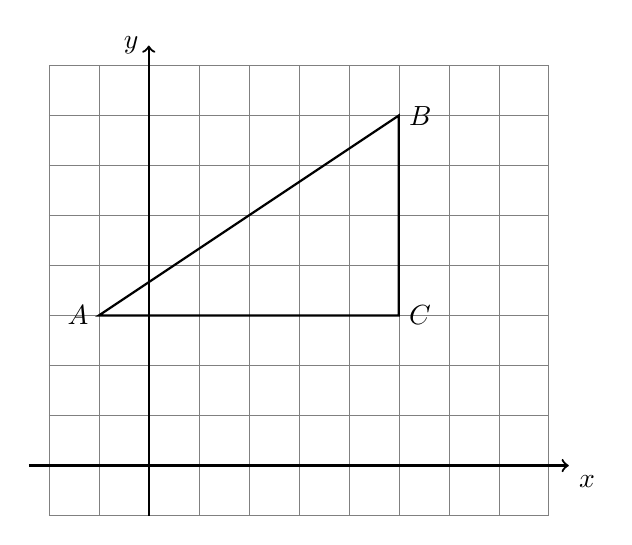
\begin{tikzpicture}[scale=.635]
            \draw [help lines] (-2,-1) grid (8,8);
            \draw [thick, ->] (-2.4,0) -- (8.4,0) node [below right] {$x$};
            \draw [thick, ->] (0,-1)--(0,8.4) node [left] {$y$};
            \draw [thick] (-1,3)node[left]{$A$}--
            (5,7)node[right]{$B$}--
            (5,3)node[right]{$C$}--
            cycle;
          \end{tikzpicture}
          \end{center}
      \end{multicols}
    \end{enumerate}
    \vspace{1cm} 

\newpage
  \item As shown, $\overline{AB}$ has endpoints with coordinates $A(-2,-3)$ and $B(6, 5)$. Show the calculation for the coordinates of the midpoint $M$ of $\overline{AB}$. Mark and label it on the graph. \hfill (2 stars)
      \begin{flushright} %4 quadrant regents grid
        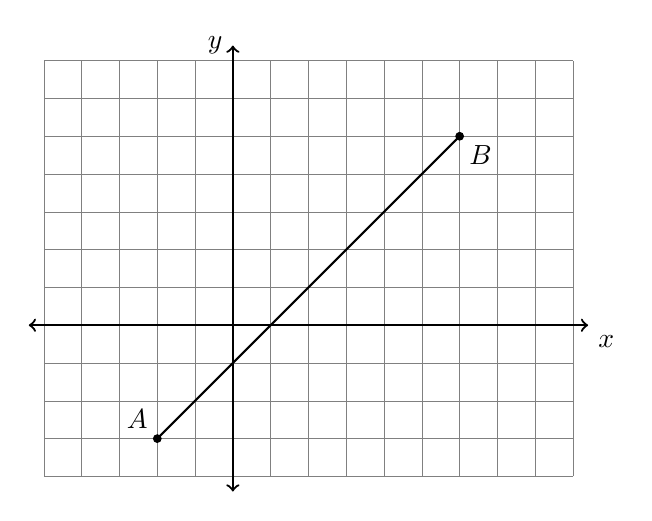
\begin{tikzpicture}[scale=.48]
          \draw [help lines] (-5,-4) grid (9,7);
          \draw [thick, <->] (-5.4,0) -- (9.4,0) node [below right] {$x$};
          \draw [thick, <->] (0,-4.4)--(0,7.4) node [left] {$y$};
          \draw [thick] (-2,-3)--(6,5);
          \draw [fill] (-2,-3) circle [radius=0.1] node[above left] {$A$};
          \draw [fill] (6,5) circle [radius=0.1] node[below right] {$B$};
        \end{tikzpicture}
      \end{flushright}

  \item $A(1,2)$ is one endpoint of $\overline{AB}$. The segment's midpoint is $M(4,3)$. Find the other endpoint, $B$.  \hfill (3 stars)
  \begin{multicols}{2}
    What translation maps \\[0.25cm] $A(1,2) \rightarrow M(4,3)$?
    \begin{flushright} %4 quadrant regents grid
      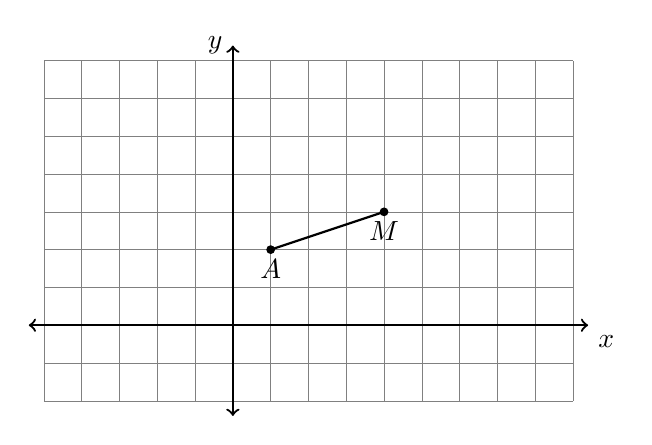
\begin{tikzpicture}[scale=.48]
        \draw [help lines] (-5,-2) grid (9,7);
        \draw [thick, <->] (-5.4,0) -- (9.4,0) node [below right] {$x$};
        \draw [thick, <->] (0,-2.4)--(0,7.4) node [left] {$y$};
        \draw [thick] (1,2)--(4,3);
        \draw [fill] (1,2) circle [radius=0.1] node[below] {$A$};
        \draw [fill] (4,3) circle [radius=0.1] node[below] {$M$};
      \end{tikzpicture}
    \end{flushright}
  \end{multicols}

  \item In the diagram below, $\overline{AD}$ has endpoints with coordinates $A(-4,-2)$ and $D(5, 4)$. What points $B$ and $C$ trisect $\overline{AD}$ into three congruent segments? Mark and label them on the graph. State their coordinates.  \hfill (3 stars)
    \begin{flushright} %4 quadrant regents grid
      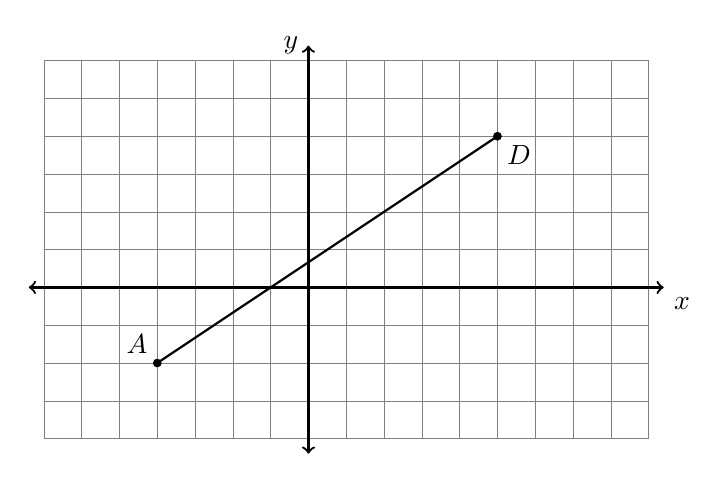
\begin{tikzpicture}[scale=.48]
        \draw [help lines] (-7,-4) grid (9,6);
        \draw [thick, <->] (-7.4,0) -- (9.4,0) node [below right] {$x$};
        \draw [thick, <->] (0,-4.4)--(0,6.4) node [left] {$y$};
        \draw [thick] (-4,-2)--(5, 4);
        \draw [fill] (-4,-2) circle [radius=0.1] node[above left] {$A$};
        \draw [fill] (5, 4) circle [radius=0.1] node[below right] {$D$};
      \end{tikzpicture}
    \end{flushright}

\end{enumerate}
\end{document}